%
% This is the LaTeX template file for lecture notes for EE 382C/EE 361C.
%
% To familiarize yourself with this template, the body contains
% some examples of its use.  Look them over.  Then you can
% run LaTeX on this file.  After you have LaTeXed this file then
% you can look over the result either by printing it out with
% dvips or using xdvi.
%
% This template is based on the template for Prof. Sinclair's CS 270.

\documentclass[twoside]{article}
\usepackage{graphics}
\setlength{\oddsidemargin}{0.25 in}
\setlength{\evensidemargin}{-0.25 in}
\setlength{\topmargin}{-0.6 in}
\setlength{\textwidth}{6.5 in}
\setlength{\textheight}{8.5 in}
\setlength{\headsep}{0.75 in}
\setlength{\parindent}{0 in}
\setlength{\parskip}{0.1 in}

%
% The following commands set up the lecnum (lecture number)
% counter and make various numbering schemes work relative
% to the lecture number.
%
\newcounter{lecnum}
\renewcommand{\thepage}{\thelecnum-\arabic{page}}
\renewcommand{\thesection}{\thelecnum.\arabic{section}}
\renewcommand{\theequation}{\thelecnum.\arabic{equation}}
\renewcommand{\thefigure}{\thelecnum.\arabic{figure}}
\renewcommand{\thetable}{\thelecnum.\arabic{table}}

%
% The following macro is used to generate the header.
%
\newcommand{\lecture}[4]{
   \pagestyle{myheadings}
   \thispagestyle{plain}
   \newpage
   \setcounter{lecnum}{#1}
   \setcounter{page}{1}
   \noindent
   \begin{center}
   \framebox{
      \vbox{\vspace{2mm}
    \hbox to 6.28in { {\bf EE 382C/361C: Multicore Computing
                        \hfill Fall 2016} }
       \vspace{4mm}
       \hbox to 6.28in { {\Large \hfill Lecture #1: #2  \hfill} }
       \vspace{2mm}
       \hbox to 6.28in { {\it Lecturer: #3 \hfill Scribe: #4} }
      \vspace{2mm}}
   }
   \end{center}
   \markboth{Lecture #1: #2}{Lecture #1: #2}
   %{\bf Disclaimer}: {\it These notes have not been subjected to the
   %usual scrutiny reserved for formal publications.  They may be distributed
   %outside this class only with the permission of the Instructor.}
   \vspace*{4mm}
}

%
% Convention for citations is authors' initials followed by the year.
% For example, to cite a paper by Leighton and Maggs you would type
% \cite{LM89}, and to cite a paper by Strassen you would type \cite{S69}.
% (To avoid bibliography problems, for now we redefine the \cite command.)
% Also commands that create a suitable format for the reference list.
\renewcommand{\cite}[1]{[#1]}
\def\beginrefs{\begin{list}%
        {[\arabic{equation}]}{\usecounter{equation}
         \setlength{\leftmargin}{2.0truecm}\setlength{\labelsep}{0.4truecm}%
         \setlength{\labelwidth}{1.6truecm}}}
\def\endrefs{\end{list}}
\def\bibentry#1{\item[\hbox{[#1]}]}

%Use this command for a figure; it puts a figure in wherever you want it.
%usage: \fig{NUMBER}{SPACE-IN-INCHES}{CAPTION}
\newcommand{\fig}[3]{
			\vspace{#2}
			\begin{center}
			Figure \thelecnum.#1:~#3
			\end{center}
	}
% Use these for theorems, lemmas, proofs, etc.
\newtheorem{theorem}{Theorem}[lecnum]
\newtheorem{lemma}[theorem]{Lemma}
\newtheorem{proposition}[theorem]{Proposition}
\newtheorem{claim}[theorem]{Claim}
\newtheorem{corollary}[theorem]{Corollary}
\newtheorem{definition}[theorem]{Definition}
\newenvironment{proof}{{\bf Proof:}}{\hfill\rule{2mm}{2mm}}

% **** IF YOU WANT TO DEFINE ADDITIONAL MACROS FOR YOURSELF, PUT THEM HERE:

\begin{document}
%FILL IN THE RIGHT INFO.
%\lecture{**LECTURE-NUMBER**}{**DATE**}{**LECTURER**}{**SCRIBE**}
\lecture{2}{August 30}{Vijay Garg}{Doyoung Kim}
%\footnotetext{These notes are partially based on those of Nigel Mansell.}

% **** YOUR NOTES GO HERE:

% Some general latex examples and examples making use of the
% macros follow.  
%**** IN GENERAL, BE BRIEF. LONG SCRIBE NOTES, NO MATTER HOW WELL WRITTEN,
%**** ARE NEVER READ BY ANYBODY.
\section{Review of Last Lecture}
\centerline{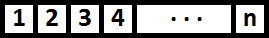
\includegraphics{1toN.png}}
Let's say there is an array with $n$ unique, unsigned integers.
If you want to find the max of array, what kind of algorithm would you use to find the max with fastest time and with least amount of work?

\subsection{Basic Sequential Algorithm}
How about good ol' sequential algorithm?
First, assume that integer on index 0 is the max. (Let's say we store the value in the variable called \textit{tempMax})
Then, compare \textit{tempMax} with another integer on the next index.
Only if `another integer' is greater than \textit{tempMax}, simply replace \textit{tempMax}'s value with `another integer'.
Continue incrementing the index until the end.
This algorithm has execution time of $O(n)$ and work load of $O(n)$.

\subsection{Binary Algorithm}
Another way is to compare integers by pairs.
First, compare integers by pairs; first thread compares index 0 and 1, second thread compares index 2 and 3, and so on.
Next, compare greater-of-twos by pairs; if index 0 was greater than index 1 and index 3 was greater than index 2, compare index 0 and index 3.
Repeat until you get the max.
This algorithm has execution time of $O(log(n))$ and work load of $O(n)$.

\subsection{All Pair Comparison Algorithm}
Now, what if you were given huge amounts of threads, let's say $n^2$?
Now, make threads to check all possible, unique combinations and change the value to 0, if value is less than other value.
After one run, there will be only one non-zero value and that is the max.
This algorithm has execution time of $O(1)$, but work load of $O(n^2)$.

\section{Ways to Create Threads in Java}
There are multiple ways to create threads in Java:
\begin{itemize}
	\item Extend {\bf Thread} -$>$ Overwrite method {\bf run()} -$>$ Call method {\bf start()} (ex. Fibonacci.java)
	\item Implement {\bf Runnable} -$>$ Overwrite {\bf run()} -$>$ Create Thread -$>$ Call {\bf start()} (ex. FooBar.java)
	\item Implement {\bf Callable} -$>$ Overwrite {\bf call()} -$>$ Use {\bf ExecutorService} class to start (ex. Fibonacci2.java)
	\item Extend {\bf RecursiveTask} -$>$ Overwrite {\bf compute()} -$>$ Use {\bf ForkJoinPool} class (ex. Fibonacci3.java)
\end{itemize}
Note that {\bf Thread} and {\bf Runnable}'s {\bf run()} do not return anything, while {\bf Callable}'s {\bf call()} and {\bf RecursiveTask}'s {\bf compute()} do.

{\bf ExecutorService} object lets program to handle the threads, rather than programmer manually handling the threads.
Combination of {\bf RecursiveTask} and {\bf ForkJoinPool} also make program to handle the threads.
Unlike {\bf ExecutorService}, {\bf RecursiveTask} enables threads to work on other job as waiting for other value(s).

Threads could be {\bf join}ed and those threads wait until all joined threads complete their tasks.
{\bf Future} class could be also used, instead of {\bf join}. {\bf Future} class lets thread to run and stops only when program needs computed value.

\section{Amdahl's Law}
Let's say, we have large tasks to complete.
If we can define ${\bf p}$, a fraction of the work that can be parallelized, we can calculate the limit on speedup for this task by Amdahl's Law.
Say, ${\bf n}$ is number of cores, ${\bf T_p}$ is time on multicore machine, and ${\bf T_s}$ is time on sequential process.
By Amdahl's Law, we get following formula:
\[{\bf T_p \ge (1-p)T_s + \frac{pT_s}{n} }\]

Which can be used to derive function for {\bf Speedup}:
\[{\bf \frac{T_s}{T_p} \le \frac{1}{1 - p + \frac{p}{n}} }\]

\section{Mutual Exclusion}
Suppose there are two threads that are doing same task, using same variable $x$ with initial value of 0 :

\noindent\begin{minipage}[t]{0.5\linewidth}
    \centering
    ${\bf T_1}$
    \[x = x + 1\]
    \end{minipage}%
    \begin{minipage}[t]{0.5\linewidth}
    \centering
    ${\bf T_2}$
    \[x = x + 1\]
\end{minipage}\par\bigskip
If those two tasks are executed at the same time, what will $x$ be after the execution?

Answer is 1. Why not 2? It is because this process is not atomic.
Because both threads were executed at the same time without variable locking or any check, when they started to run, they both see the initial value of $x$, which is 0.
Both tasks, then, will add 1 to the value they saw, and store it to variable $x$.
Conditions such as this, where more than one threads may read and write on same variable at the same time, is called {\bf critical section}. To avoid {\it critical section}, code has to be executed atomically.

\subsection{Door Problem}
Assume there are two threads, $P_1$ and $P_2$ trying to use same 'door'.

\noindent\begin{minipage}[t]{0.5\linewidth}
    \centering
    ${\bf P_0}$
    
    loop
    
    ----- Entry -----
    
    Critical Section (CS)
    
    ----- Exit -----
    
    Not Critical Section (NCS)
    
    Go back to loop
    \end{minipage}%
    \begin{minipage}[t]{0.5\linewidth}
    \centering
    ${\bf P_1}$
    
    loop
    
    ----- Entry -----
    
    Critical Section (CS)
    
    ----- Exit -----
    
    Not Critical Section (NCS)
    
    Go back to loop
\end{minipage}\par\bigskip
If two threads are executed at the same time, how can we prevent {\it critical section}?

How about using a variable to keep track of the door (Ex. Attempt1.java)?
In this process, each thread checks whether door is open or not by looking at boolean variable {\it openDoor}.
While {\it openDoor} is false, wait until it becomes true.
If {\it openDoor} is true, set it to false and then execute code.
After all necessary lines are executed, set {\it openDoor} back to true.
This attempt does not work, because threads may check {\it openDoor} at the same time before any one thread sets {\it openDoor} to false.

How about using two variables instead of one (Ex. Attempt2.java)?
In this process, there is a boolean array {\it wantCS} and each index of {\it wantCS} is assigned to all threads ($P_0$ gets index 0 and $P_1$ gets index 1).
A thread sets its corresponding {\it wantCS} to true, right before it checks whether other thread wants or not,  
This attempt does not work, because if both threads set their {\it wantCS} to true, none of both threads threads will be able to get past while loop.
This situation, which all threads are stuck in some part of the code, is called {\bf deadlock}.

How about manually setting which thread goes first (Ex. Attempt3.java)?
In this process, $P_0$ will execute its code first and then let $P_1$ to execute.
After $P_1$ executes its code, it will let $P_0$ to execute.
This attempt does work, but since threads don't know whether other thread needs to execute or not, there may be unnecessary waiting time.

\subsection{Peterson's Algorithm}
Peterson's Algorithm (Ex. PetersonAlgorithm.java) uses approaches of Attempt2 and Attempt3 ({\it wantCS} and {\it turn}).
This process gives each thread a turn, but also checks whether that thread wants to execute the code or not.

{\bf Check for Deadlock Freedom}
\[Deadlock \equiv (wantCS[1] \wedge turn == 1) \wedge (wantCS[0] \wedge turn == 0)\]
\[\Rightarrow turn == 1 \wedge turn == 0\]
\[\Rightarrow false\]
{\bf Check for Mutual Exclusion}\\
Let's add another boolean array, {\it trying}.
Only when thread is checking for while-loop conditions, corresponding index of {\it trying} becomes true.
Otherwise, it is false.

Consider predicate H, where:
\[H(0) \equiv wantCS[0] \wedge [(turn == 1) \vee ((turn == 0) \wedge trying[1])]\]
\[H(1) \equiv wantCS[1] \wedge [(turn == 0) \vee ((turn == 1) \wedge trying[0])]\]

In here, $P_0$ cannot falsify $H(1)$.
Because only $P_1$ can change the value of wantCS[1], $H(1)$ will be falsified only if $wantCS[1] \wedge turn == 1 \wedge trying[0]$ holds true.
When $turn$ is set to 1 by $P_0$, trying[0] is false. From symmetry, $P_1$ also cannot falsify $H(0)$.

Now, check for the mutual exclusion:
\[Critical Section \equiv \neg trying[0] \wedge H(0) \wedge \neg trying[1] \wedge H(1)\]
\[\Rightarrow turn == 0 \wedge turn == 1\]
\[\Rightarrow false\]


\section*{References}
\beginrefs
\bibentry{1}{\sc V. K. ~Garg},
 Introduction to Multicore Computing,
pp.~21-22.
\endrefs


\end{document}





